\documentclass{beamer}
%\documentclass[handout]{beamer}
\usetheme{Antibes}

\usepackage{fontspec}
\usepackage[catalan]{babel}
\usepackage{hyperref}
\usepackage[normalem]{ulem}
\usepackage{tikz}
\usepackage{listings}

\input{python.tex}

\AtBeginSection[]
{
	\begin{frame}{Contingut}
		\tableofcontents[currentsection]
	\end{frame}
}

\title{Construcció d'una orquestra amb Raspberry Pi}
\author{Arnau Canyadell Miquel \and Joan Marcè Igual}
\date{2 de Juny de 2017}

\begin{document}

\frame{\titlepage}
\section{Introducció}
\begin{frame}{Descripció del projecte}
	Crear amb Raspberry Pi una orquestra musical formada per un director i uns quants músics que interpreten el que els mana el director.
	\begin{figure}
		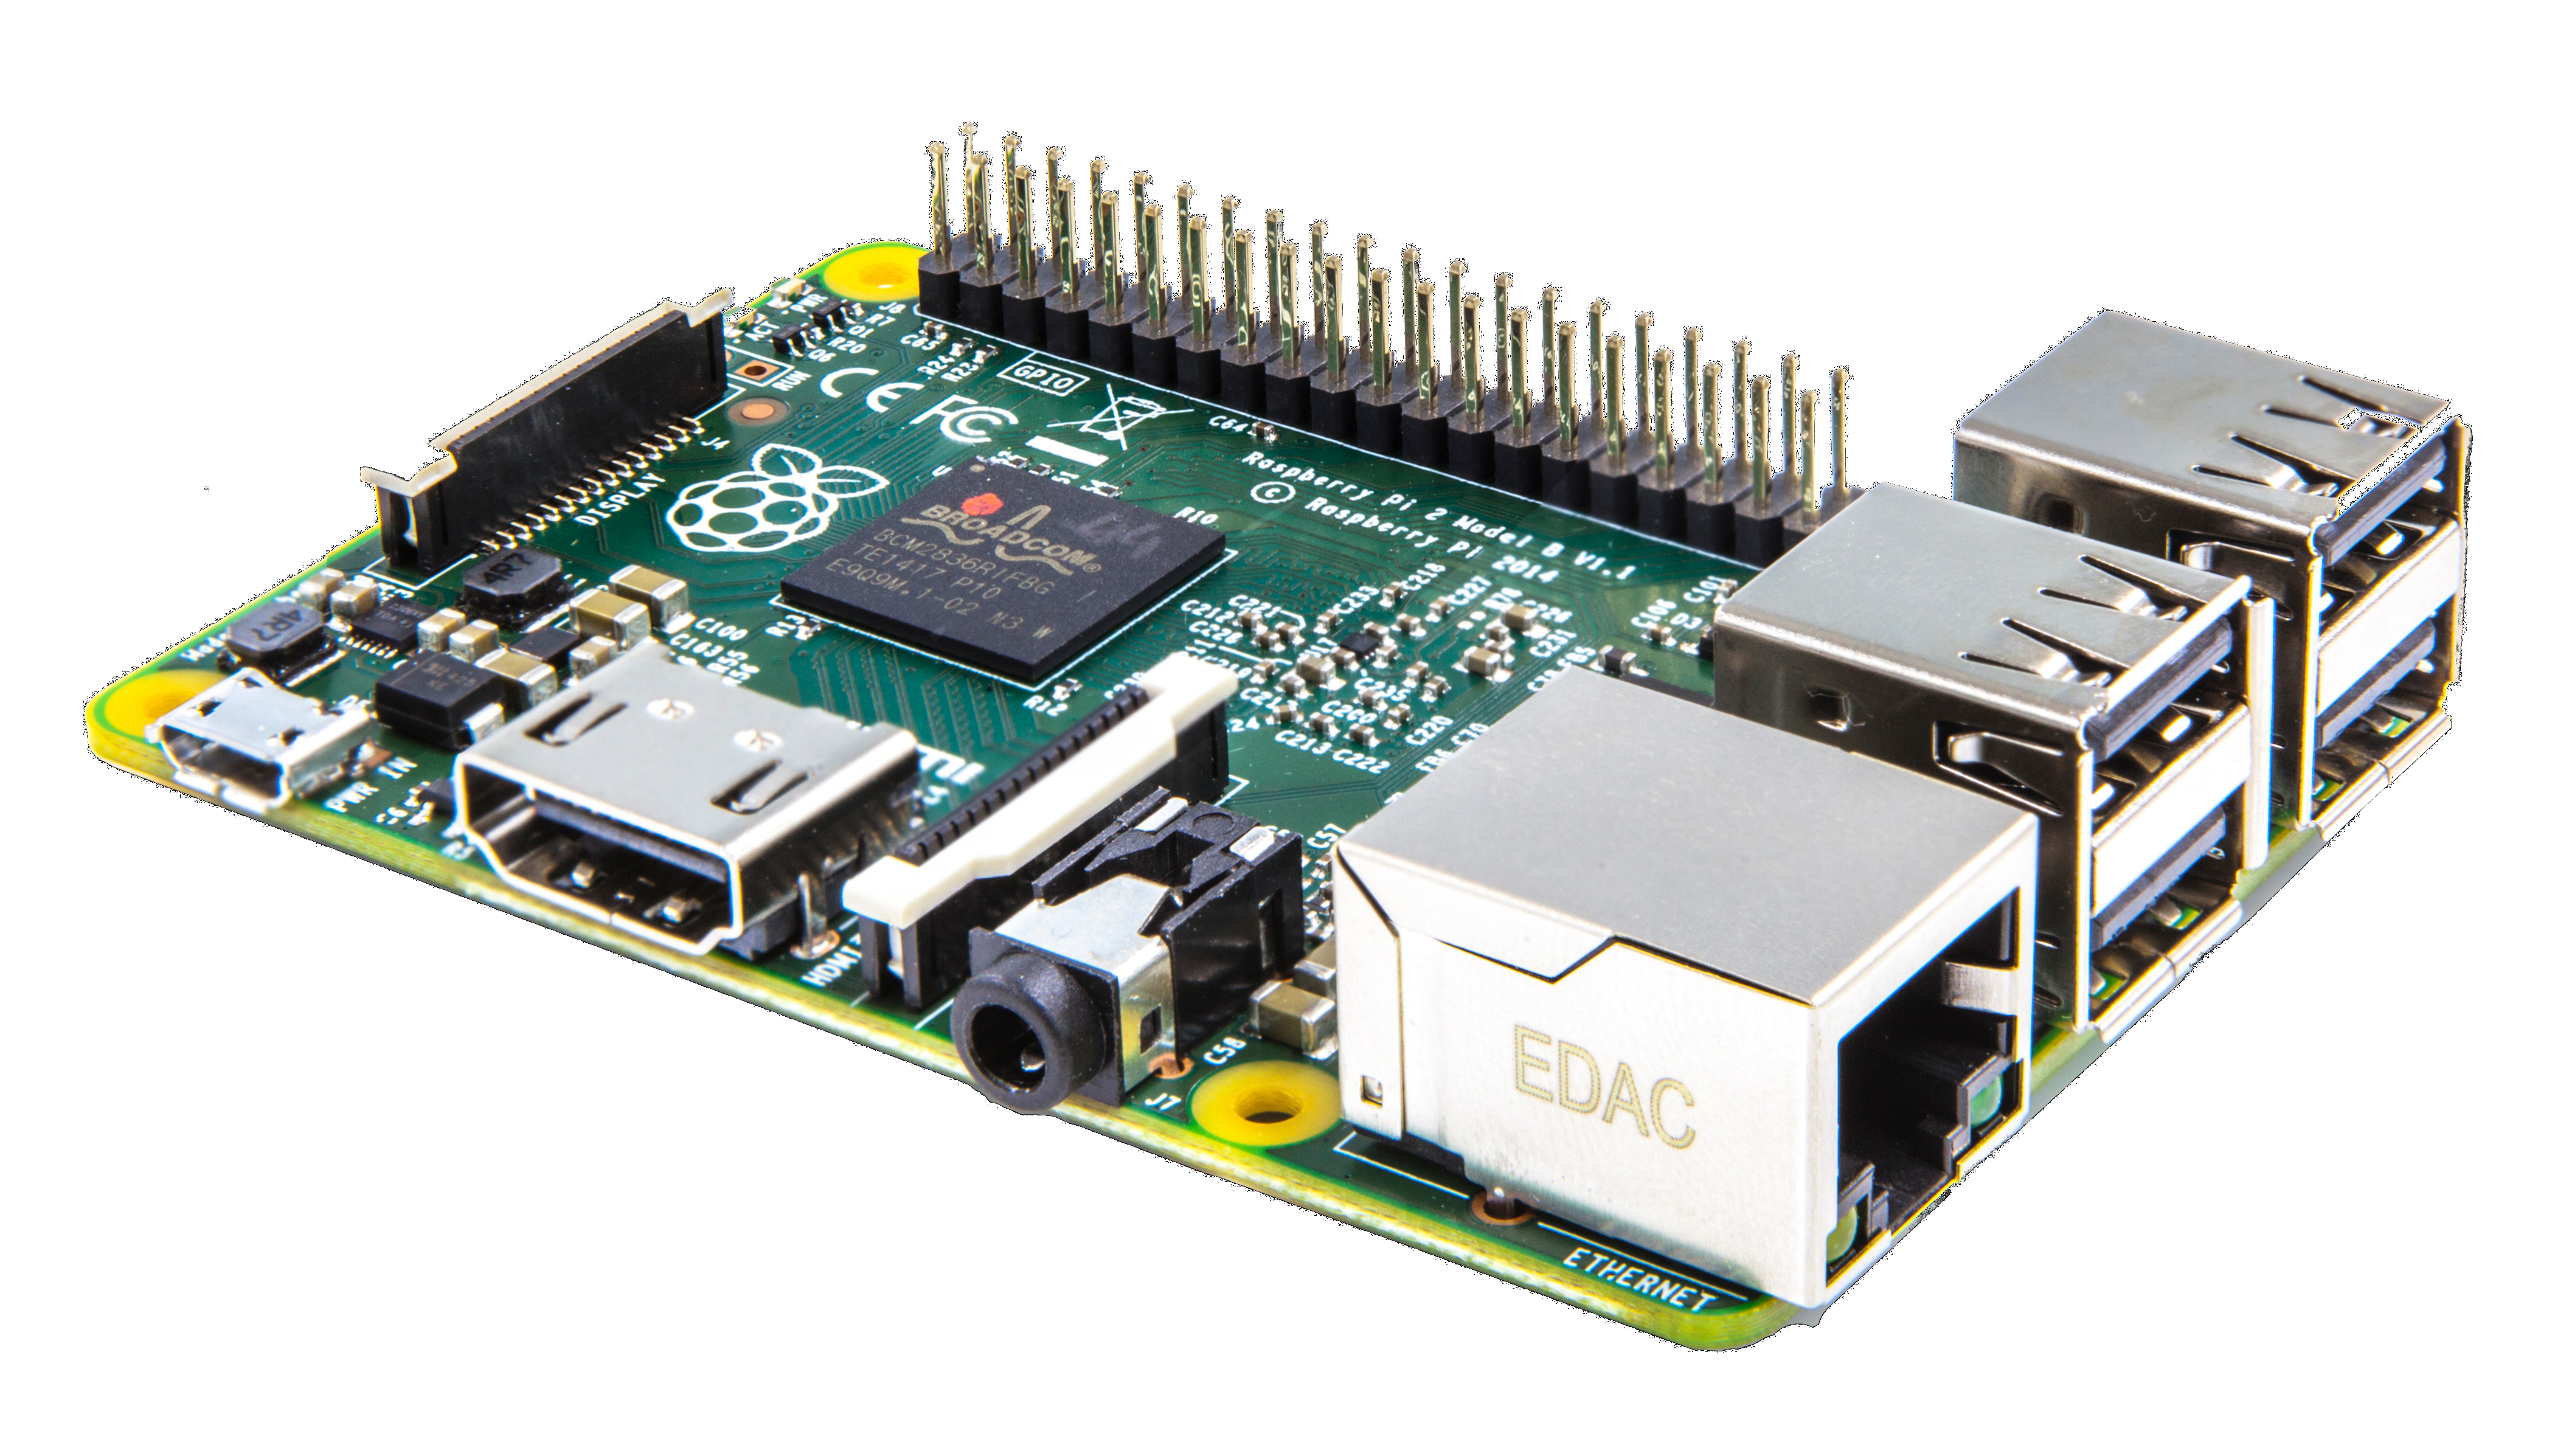
\includegraphics[width=0.475\linewidth]{images/raspberry}
		\hfill
		\includegraphics[width=0.475\linewidth]{images/orchestra}
	\end{figure}
\end{frame}

\section{Objectius}
\subsection{Objectius a curt termini}
\begin{frame}{Objectius a curt termini}
	
	\begin{itemize}
		\item Aconseguir rebre la música d'un ordinador
		\item Enviar la música a una Raspberry Pi
		\item Reproduir la música en una Raspberry Pi
	\end{itemize}
\end{frame}

\subsection{Objectius a llarg termini}
\begin{frame}{Objectius a llarg termini}
	\begin{itemize}
		\item Programar un bot per a l'aplicació de missatgeria Telegram que reprodueixi amb l'orquestra de Raspberry Pis la música que se li enviï.
		\item Enviar música del mòbil a l'ordinador.
	\end{itemize}
\end{frame}

\section{Feina feta}
\begin{frame}{Què hem fet fins ara?}
	\begin{itemize}
		\item Establiment dels objectius
		\item Analitzat el codi del director
		\item Programat el codi de l'intèrpret (músic)
		\item Codi per configurar una raspberry pi qualsevol per a funcionar com a músic
		\item Canvis en el codi del director
	\end{itemize}
\end{frame}

\begin{frame}
	\frametitle{Principals problemes trobats i solucionats}
	\begin{itemize}[<+->]
		\item Mida de les targetes SD. 4 GB no era suficient.
		\begin{itemize}
			\item Usar una targeta més gran
			\item Usar versió LITE de \texttt{Raspbian}
		\end{itemize}
		\item Àudio en la raspberry pi. No hem sabut canviar el dispositiu de sortida des de l'entorn de comandes. Hem hagut d'insta\l.lar l'entorn gràfic a la raspberry pi.
		\begin{itemize}
			\item Finalment trobat
			\item Crear script que canvii el dispositiu per defecte
		\end{itemize}
		\item La llibreria midi Music21 és molt lenta per llegir midi.
		\begin{itemize}
			\item Usar la llibreria \texttt{mido}.
		\end{itemize}
	\end{itemize}
\end{frame}

\section{Funcionament}
\subsection{Multicast}
\begin{frame}{Multicast}
	Prova xunga per veure perquè no funciona això

\begin{figure}[H]
	\centering
	\begin{tikzpicture}
		\node[label = below:{Router}](router){\includesvg{images/cisco/router}};
		\node[below = of router, label = below:{Switch}](switch){\includesvg{images/cisco/workgroup_switch} };
		\draw[latex-latex] (router) -- (switch);
	\end{tikzpicture}
\end{figure}
\end{frame}
\subsection{Bucle reproducció}
\begin{frame}[fragile]{Bucle de reproducció}
	\begin{lstlisting}[
			label={lst:code},
			style=mypython, 
			basicstyle=\ttfamily\tiny,
			captionpos=b,
			xleftmargin=.05\textwidth, 
			xrightmargin=.05\textwidth,
			caption={Bucle bàsic per enviar les dades de notes}
		]
	# file_path: conté el camí fins a l'arxiu
	# multicast_group: conté la ip al grup de multicast
	# La funció play_tracks() ja fa les pauses que s'hagin de fer perquè
	# les notes sonin quan toca
	mid = DirectorMidiFile(file_path)
	for missatge, track in mid.play_tracks():
		msg_in, msg_out = descodifica(missatge, track)
		# Genera string a enviar
		json_string = json.dumps({
		"in": msg_in,
		"out": msg_out
		})
		
		# Enviar dades al multicast
		socket.sendto(json_string.encode(), multicast_group)
	\end{lstlisting}
\end{frame}

\section{Demostració}
\begin{frame}{Demostració en directe}
	\begin{figure}
		\includegraphics[width=\linewidth]{images/orchestra}
	\end{figure}
\end{frame}

\end{document}